\documentclass[a4paper]{article}\usepackage[]{graphicx}\usepackage[]{color}
%% maxwidth is the original width if it is less than linewidth
%% otherwise use linewidth (to make sure the graphics do not exceed the margin)
\makeatletter
\def\maxwidth{ %
  \ifdim\Gin@nat@width>\linewidth
    \linewidth
  \else
    \Gin@nat@width
  \fi
}
\makeatother

\definecolor{fgcolor}{rgb}{0.345, 0.345, 0.345}
\newcommand{\hlnum}[1]{\textcolor[rgb]{0.686,0.059,0.569}{#1}}%
\newcommand{\hlstr}[1]{\textcolor[rgb]{0.192,0.494,0.8}{#1}}%
\newcommand{\hlcom}[1]{\textcolor[rgb]{0.678,0.584,0.686}{\textit{#1}}}%
\newcommand{\hlopt}[1]{\textcolor[rgb]{0,0,0}{#1}}%
\newcommand{\hlstd}[1]{\textcolor[rgb]{0.345,0.345,0.345}{#1}}%
\newcommand{\hlkwa}[1]{\textcolor[rgb]{0.161,0.373,0.58}{\textbf{#1}}}%
\newcommand{\hlkwb}[1]{\textcolor[rgb]{0.69,0.353,0.396}{#1}}%
\newcommand{\hlkwc}[1]{\textcolor[rgb]{0.333,0.667,0.333}{#1}}%
\newcommand{\hlkwd}[1]{\textcolor[rgb]{0.737,0.353,0.396}{\textbf{#1}}}%

\usepackage{framed}
\makeatletter
\newenvironment{kframe}{%
 \def\at@end@of@kframe{}%
 \ifinner\ifhmode%
  \def\at@end@of@kframe{\end{minipage}}%
  \begin{minipage}{\columnwidth}%
 \fi\fi%
 \def\FrameCommand##1{\hskip\@totalleftmargin \hskip-\fboxsep
 \colorbox{shadecolor}{##1}\hskip-\fboxsep
     % There is no \\@totalrightmargin, so:
     \hskip-\linewidth \hskip-\@totalleftmargin \hskip\columnwidth}%
 \MakeFramed {\advance\hsize-\width
   \@totalleftmargin\z@ \linewidth\hsize
   \@setminipage}}%
 {\par\unskip\endMakeFramed%
 \at@end@of@kframe}
\makeatother

\definecolor{shadecolor}{rgb}{.97, .97, .97}
\definecolor{messagecolor}{rgb}{0, 0, 0}
\definecolor{warningcolor}{rgb}{1, 0, 1}
\definecolor{errorcolor}{rgb}{1, 0, 0}
\newenvironment{knitrout}{}{} % an empty environment to be redefined in TeX

\usepackage{alltt}

%% Language and font encodings
\usepackage[english]{babel}
\usepackage[utf8x]{inputenc}
\usepackage[T1]{fontenc}
\usepackage{float}

%% Sets page size and margins
\usepackage[a4paper,top=3cm,bottom=2cm,left=3cm,right=3cm,marginparwidth=1.75cm]{geometry}

%% Useful packages
\usepackage{amsmath}
\usepackage{graphicx}
\usepackage[colorinlistoftodos]{todonotes}
\usepackage[colorlinks=true, allcolors=blue]{hyperref}

\title{Stat 159 Final Project - Providing Credit to Students}
\author{Team W.O.S: Yoon Jung Rho, Young Hoon Kim, Ellen Hwang, Joseph Simonian}
\IfFileExists{upquote.sty}{\usepackage{upquote}}{}
\begin{document}
\maketitle

\begin{abstract}
Our client profile is a credit institution that provides financial aid to students. The managers are interested in expanding their customer base but they would also like that most of the loans be payed back. Our team's purpose is to perform exploratory data analysis and create predictive models to find which schools and what kind schools credit institutions should provide credit.
\end{abstract}
\section{Introduction}

Our client, a credit institution that provides financial aid to students, want to expand their customer base but would also like that most of the loans be payed back. Our role as the analyst is to use the publicly available [College Scoreboard Datasets](https://collegescorecard.ed.gov/data/) to figure out what features of a college make it more reliable for credit. Our team will be using the 3 year repayment rate as am indicator of the school's overall reliability rate. Using exploratory data analysis we will examine the relationships between repayment rate and other features of the school. In our analysis, we will use ridge, lasso, partial least squares, and principle component regression to find significant features that influence a school's overall repayment rate. 
\section{Data}

The data from College Scorecard provide insights into the performance of schools eligible to receive federal financial aid, and offer a look at the outcomes of students at those schools. The Data that appear on the College Scorecard provides data on student completion, debt and repayment, earnings, and more. The files include data from 1996 through 2016 for all undergraduate degree-granting institutions of higher education. This data was last updated on September 13th, 2016. The data is available at: \url{https://collegescorecard.ed.gov/data/}

For our project, besides the main data, our team also used featured downloads provided by College Scorecard. These data downloads provide quick access to some of the data in which users may be most interested, including a file that offers the most current data for each element. Among variety of data, we used [Post-School earnings](https://ed-public-download.apps.cloud.gov/downloads/Most-Recent-Cohorts-Treasury-Elements.csv) to narrow down the analytical component.

There is also a documentation that provides more on how to use the data, including: Sources of the data, The construction of metrics, and Data considerations and limitations available at: \url{https://collegescorecard.ed.gov/data/documentation/}

\section{Methods}\section{Results}

\subsection{Correlation and Regession Results to find Relevant Variables}
WRITE SOMETHING ABOUT USING REGRESSIONS TO SELECT VARIABLES 


\subsection{Exploratory Data Analysis}
After using correlation and regression to select features related to repayment, we were able to perform some exploratory data analysis. 

\begin{figure}
  \caption{Scatter Plot of Completion Rate vs. 3 Year Repayment Rate}
  \centering
  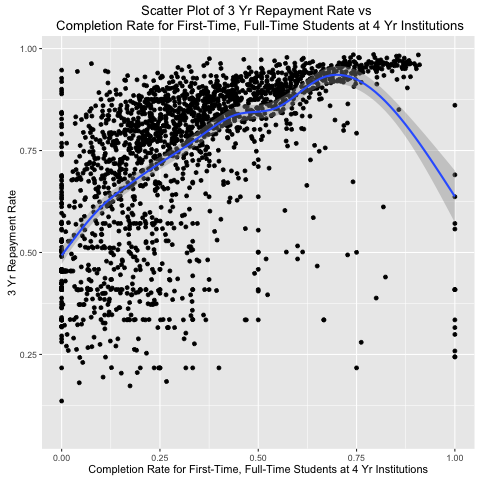
\includegraphics[width=0.6\textwidth]{../images/eda/complrt_rpy3yr_scatter.png}
  \centering
  \newline
  
  \raggedright
From the graph, we can see that schools with repayment rates below 75\% tend to have completion rates below 50\%. There is also a very steep trend for completion rate for repayment rates above 75\%. 
\end{figure}
 


\begin{figure}
  \caption{Scatter Plot of Different Tuition Types on 3 Year Repayment Rate}
  \centering
  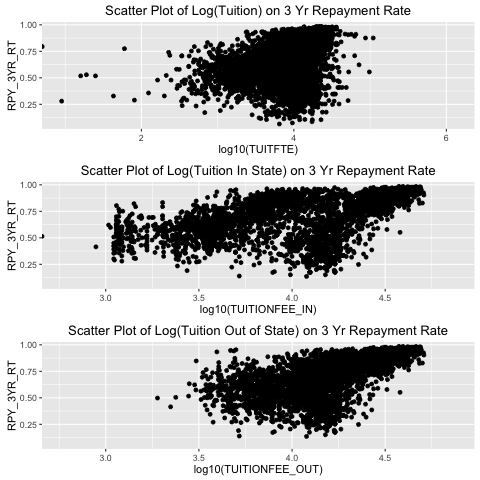
\includegraphics[width=0.6\textwidth]{../images/eda/rpy3yr_tuition_scatter.png}
  \centering
  \newline
  
  \raggedright
This figure displays three different scatterplots of Tuition fee vs Repayment Rate. In the data set, there are three different information of Tuition fee under cost category. First graph is a Net tuition revenue per full-time equivalent student vs repayment rate. Second graph is a In-stat tuition and fee vs repayment rate and last one is out-of-state tuition and fees vs repayment rate. There is highest correlation between out-of-state vs repayment rate.
\end{figure}


\begin{figure}
  \caption{Scatter Plot of 3 Year Repayment Rates on Type of Institution}
  \centering
  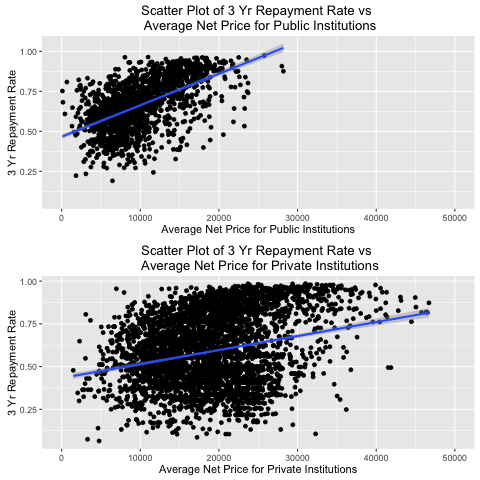
\includegraphics[width=0.6\textwidth]{../images/eda/netprice_pub_priv_rpy3yr_scatter}
  \centering
  \newline
  
  \raggedright
The figure aboce is a scatterplot of 3 Year Repayment Rate vs average net price for public institutions and below, it has a scatterplot of 3 Year Repayment Rate vs average net price for private instutitions. It shows higher slope for public institution but for both graph, it shows weak relationship between the average net price and repayment rate. 
\end{figure}


\begin{figure}
  \caption{Scatter Plot of Repayment Rates on Type of Institution}
  \centering
  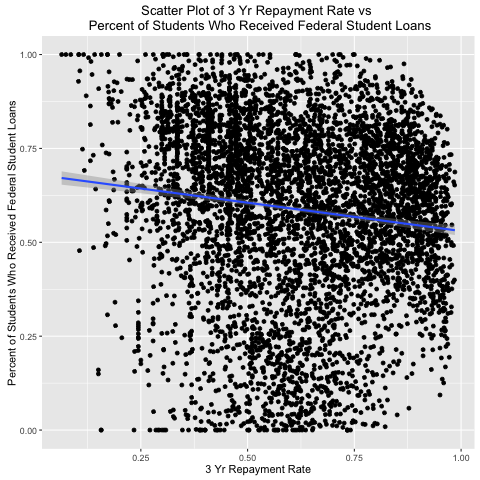
\includegraphics[width=0.6\textwidth]{../images/eda/pctfloan_rpy3yr_scatter}
  \centering
  \newline
  
  \raggedright
The figure aboce is a scatterplot of 3 Year Repayment Rate vs percent of students who received federal student loans. By looking the graph, it shows that there is weak relationship between percent of students who recieved federal student loans and 3yr repayment rate.
\end{figure}


\begin{figure}
  \caption{Barplot of Mean 3 Year Repayment Rate on REGION Levels}
  \centering
  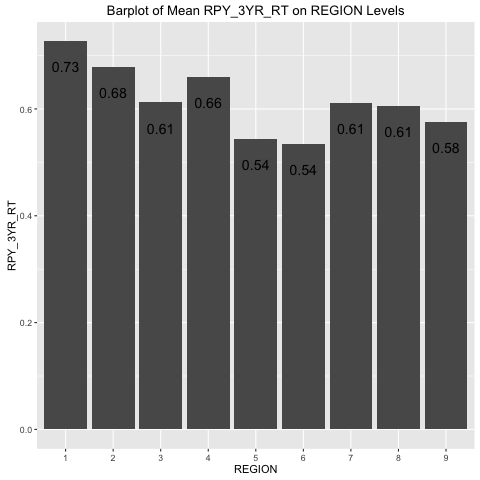
\includegraphics[width=0.6\textwidth]{../images/eda/rpy_region_barplot.png}
  \centering
  \newline
  
  \raggedright
This figure displays a barplot of average value of 3 Year Repayment Rate for each region. 3 Year Repayment Rate is defined as a fraction of repayment cohort who are not in default, and with loan balances that have declined three years since entering repayment, excluding enrolled and military deferment from calculation. (rolling averages) and each university is divided into 9 regions: 0	U.S. Service Schools, 1New England (CT, ME, MA, NH, RI, VT), 2	Mid East (DE, DC, MD, NJ, NY, PA), 3	Great Lakes (IL, IN, MI, OH, WI),4	Plains (IA, KS, MN, MO, NE, ND, SD), 5	Southeast (AL, AR, FL, GA, KY, LA, MS, NC, SC, TN, VA, WV), 6	Southwest (AZ, NM, OK, TX), 7	Rocky Mountains (CO, ID, MT, UT, WY), 8	Far West (AK, CA, HI, NV, OR, WA), 9	Outlying Areas (AS, FM, GU, MH, MP, PR, PW, VI). Our graph is not showing region 0 because there is one university that is under region 0 and it did not have a value for 3 Year Repayment Rate On barplot it shows that region 1 and 2 have highest repayment rate(0.73 and 0.68, respectively) and region 5 and 6 have lowest repayment rate (0.54)
\end{figure}


\begin{figure}
  \centering
  \caption{Barplot of Mean 3 Year Repayment Rate on Control Levels and Distributions of 3 Year Repayment Rate for Control Level}
  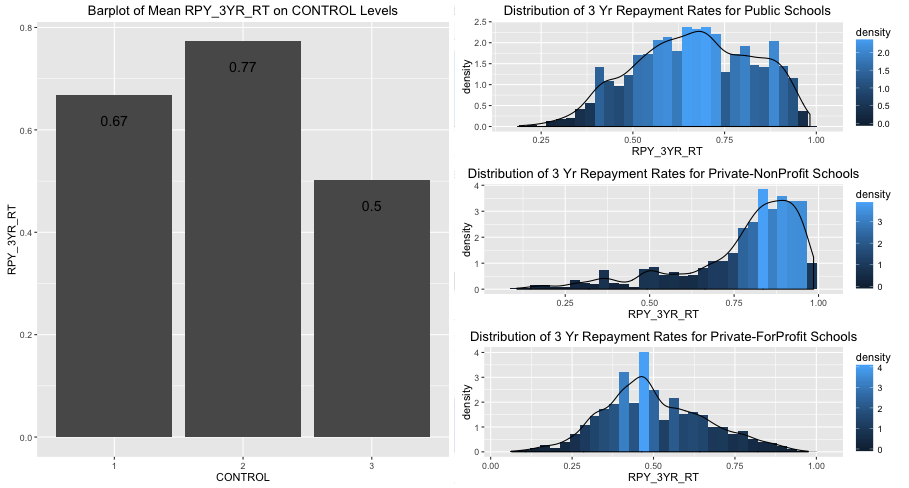
\includegraphics[width=0.6\textwidth]{../images/eda/rpy3yr_control_barplot_histogram.png}
  \centering
  \newline
  
  \raggedright
This figure displays a barplot that shows average value of 3 Year Repayment Rate for each school type. Under Control column, each school is divided into three categories: 1 = Public, 2 = Private nonprofit, 3 = Private for-profit. It shows that Private for nonprofit universities has highest average repayment rate with 0.77. On the right side, histogram helps for the better understanding of barplot. The visualizations on the right shows density graph and histogram of each institution's repayment rate.
\end{figure}


\begin{figure}
  \caption{Barplot of Mean 3 Year Repayment Rate on ICLEVEL Levels and Distributions of 3 Year Repayment Rate for each ICLEVEL Level}
  \centering
  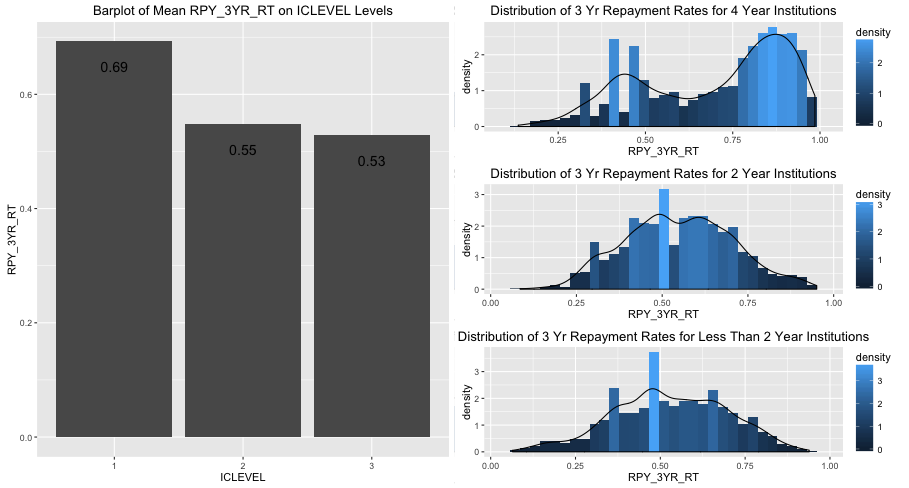
\includegraphics[width=0.6\textwidth]{../images/eda/iclevel_rpy3yr_barplot_histogram.png}
  \centering
  \newline
  
  \raggedright
This figure is a barplot that shows average value of 3 Year Repayment Rate for each level of institution. Uncer ICLEVEL, each school is divided into three categories: 1 = 4-year,2 = 2-year, 3 = Less-than-2-year. It shows that 4-year institution has the highest average repayment rate with 0.69. On the right side of the barplot, there is a histogram/desnity plot of each institution's repayment rate for detailed analysis.
\end{figure}



\section{Analysis}

\begin{table}[!h]
\centering
\caption{Top 10 Schools} 
\begin{tabular}{rlr}
  \hline
 & INSTNM & row\_mean \\ 
  \hline
443331 & West Coast University-Los Angeles & 1.02 \\ 
  167996 & Stonehill College & 0.99 \\ 
  217165 & Bryant University & 0.99 \\ 
  213251 & Juniata College & 0.99 \\ 
  177719 & Barnes-Jewish College Goldfarb School of Nursing & 0.99 \\ 
  211440 & Carnegie Mellon University & 0.99 \\ 
  239716 & Saint Norbert College & 0.98 \\ 
  152080 & University of Notre Dame & 0.98 \\ 
  181428 & University of Nebraska Medical Center & 0.98 \\ 
  216524 & Ursinus College & 0.98 \\ 
   \hline
\end{tabular}
\end{table}

\section{Conclusions}


\end{document}
